\documentclass{article}

\usepackage[margin=1in]{geometry}     %for 1inch margins that play nice with fancyhdr
\usepackage{amsmath,amssymb}          % math and junk
\usepackage{fancyhdr}                 % for a nice running header and footer
\usepackage{lastpage}                 % for nice "X of Y" footer
\usepackage[per-mode=symbol,alsoload=binary,detect-all=true]{siunitx}
                                      % for nice units and junk!
\usepackage{gnuplot-lua-tikz}         % enable tikz plots made from gnuplot
\usepackage{float}                    % [H] option for floats
\usepackage[american]{circuitikz}     % for teh circuit diagrams
\usepackage[hidelinks]{hyperref}                 % get those sweet, sweet, links
\usepackage{framed}                   % for framed titlepage
\usepackage{subfig}

\usetikzlibrary{shapes,arrows}

% unused, but common for other experiments
%\usepackage{rotating}                 % for sideways stuff!
%\usepackage{cancel}                   % for `canceling out' parts of equations. fancy!
\usepackage{mdwlist}                  % itemize* and friends
%\usepackage{verbatim}                 % for \verbatiminput command and comment environment
%\usepackage[colorinlistoftodos]{todonotes}                % todo's, if used/needed
%\usepackage{multirow}                 % for multi-row spans in tabular environment


% values!
\newcommand{\docAuthor}{Sean Barag}
\newcommand{\docCoAuthor}{None}
\newcommand{\ta}{Yang Gao}
\newcommand{\docTitle}{ADC and DAC Simulations}
\newcommand{\courseName}{ECE-L304}
\newcommand{\labNum}{Step 1}
\newcommand{\labSec}{064}
\newcommand{\dueDate}{20 January 2012}
\newcommand{\perfDate}{11 January 2012}

% paths
\graphicspath{{$HOME/texmf/graphics/}}


% meta-data
\pdfinfo{
	/Title    (\labNum: \docTitle)
	/Author   (\docAuthor)
	/Keywords (\docTitle, \labNum)
}

% for fancy header
\pagestyle{fancy}
\lhead{\courseName\ $|$ \labSec}
\chead{\labNum: \docTitle}
\rhead{\docAuthor}
\cfoot{\thepage\ of \pageref{LastPage}}

% title info
\title{\courseName\ \labNum: \\ \docTitle}
\author{\docAuthor}
\date{}

% shortcuts, cause I'm lazy
\newcommand{\bs}[1]{\boldsymbol{#1}}
\newcommand{\tbf}[1]{\textbf{#1}}
\newcommand{\ttt}[1]{\texttt{#1}}

\begin{document}
% Cover page written by Bryndon Blackburn
% Originally written by Bryndon Blalckburn
\begin{titlepage}
	\begin{center}
		\includegraphics[scale = 0.50]{DrexelLogo.pdf}
	\end{center}

	\large
	\begin{framed}
		\begin{center}
			Electrical and Computer Engineering Dept. \\
			Electrical Engineering Laboratory IV, ECE-L304 \\
		\end{center}
	\end{framed} \vspace{50pt}

	\begin{description}
		\item[Title:]\labNum: \docTitle
		\item[Author:] \docAuthor
		\item[Partner:] \docCoAuthor
		\item[Instructor:] \ta
		\item[Section:] \labSec
		\item[Date Performed:] \perfDate
		\item[Date Due:] \dueDate
		\item[Date Received:]
	\end{description}
\end{titlepage}


% Blank page so two-sided printing leaves the cover page on its own sheet
\thispagestyle{empty}
\newpage
\mbox{}

\maketitle
\setcounter{page}{1} % fixes page numbering issues caused by cover sheet
\tableofcontents % this helps
\newpage
\listoffigures   % there's over 9000 figures

\newpage % I want the actual content to be at the top of a new page
\section{Introduction}
The entirety of ECE-L304 is devoted to the design, construction, and debugging
of a digital voice recorder.  By providing students with an opportunity to
complete a project of larger scale than anything they have previously
attempted, the course offers its students valuable skills and experience with a
long-term engineering project.

As the system uses digital storage in the form of a RAM chip, it is necessary
to convert all input audio from its native analog form to a digital
representation.  Similarly, the stored digital representation must be converted
back to an analog signal so that it can be correctly rendered by a speaker.
These conversions are performed by an analog to digital converter (ADC) and a
digital to analog converter (DAC), resepectively.
%
In order to ease the design process, students first complete a simple ADC and
DAC simulation.  This helps to remind students of the operating properties and
behaviors of the two converters, as well as providing a schematic similar to
the one required in the final design.

\section{Digital to Analog Converter}
\subsection{Prediction}
% TODO: Prediction graph

\subsection{Discrete DAC}
The provided DAC schematic was captured in Cadence PSpice as shown in
Figure~\ref{f:dac_schem}.
%
\begin{figure}[H]
\centering
	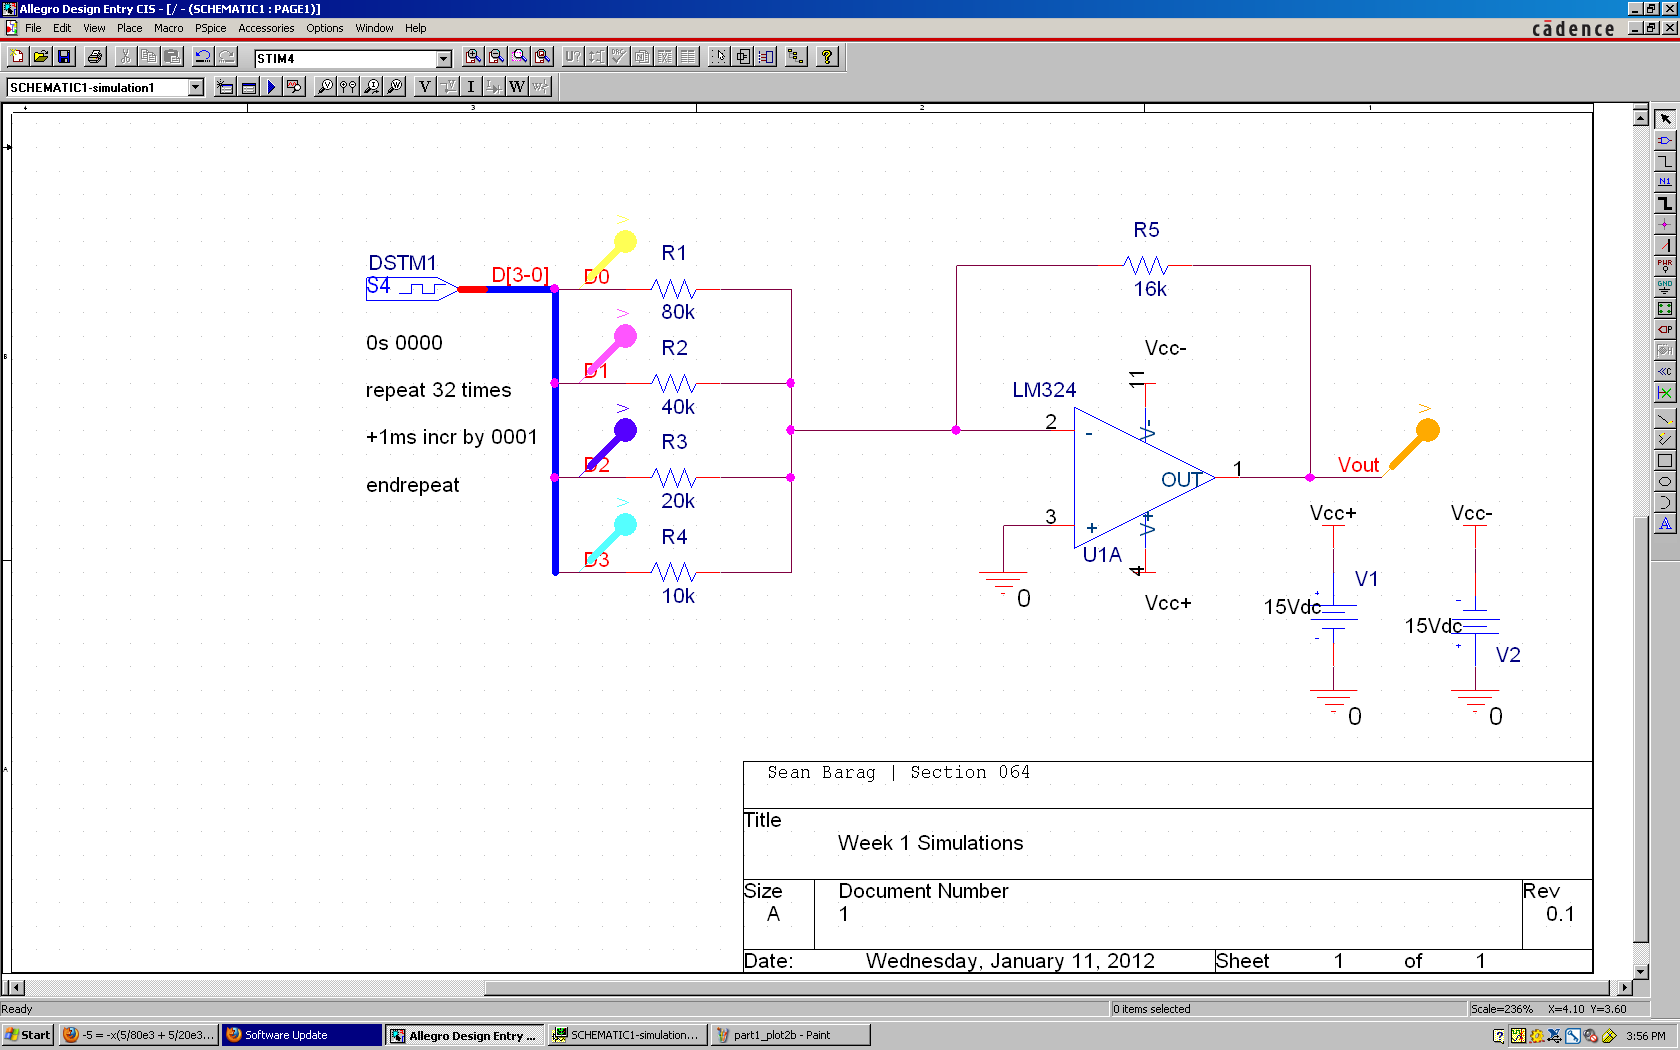
\includegraphics[width=.8\textwidth]{img/shot/part1_schem.PNG}
	\parbox{.8\textwidth}{
	\caption[Discrete DAC --- Schematic]{Provided schematic for the discrete
	digital to analog converter (DAC).  Note that the value of~$R_5$ has
	already been adjusted in this image.}
	\label{f:dac_schem}}
\end{figure}
%
Note that the element titled ``DTSM 1'' was edited to repeatedly count from
zero~($0000_2$) to fifteen~($1111_2$) with each intermediate value
lasting for~\SI{1}{\milli\second}.  This was accomplished by editing the
element properties and providing the four instructions shown:
%
\begin{itemize*}
	\item \ttt{0s 0000}
	\item \ttt{repeat 32 times}
	\item \ttt{+1ms incr by 00001}
	\item \ttt{endrepeat}
\end{itemize*}
%
This circuit was simulated using transient analysis for the
required~\SI{32}{\milli\second}, allowing one full input count-up cycle to be
observed.  The voltage at each bit, along with the output voltage, is plotted
below in Figure~\ref{f:dac_plot1}.
%
\begin{figure}[H]
\centering
	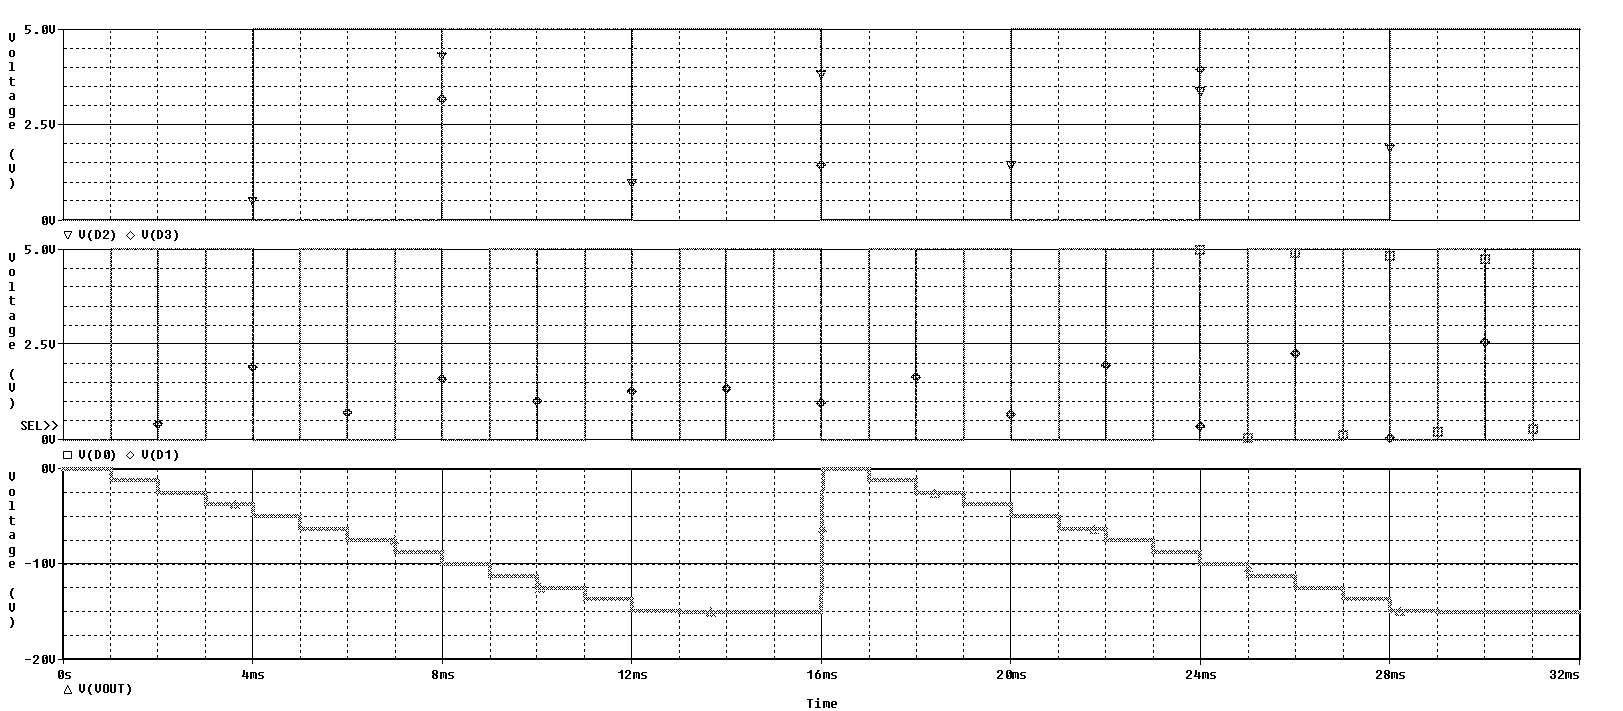
\includegraphics[width=.8\textwidth]{img/plot/part1_plot1b.PNG}
	\parbox{.8\textwidth}{
	\caption[Discrete DAC --- Initial Results]{Initial simulation results for
	the discrete DAC.  Note that the output reaches a lower threshold as a
	result of the value of~$R_5$.}
	\label{f:dac_plot1}}
\end{figure}
%
As is shown in the produced plot of output voltage versus time, the output
reaches the minimum possible output voltage of~\SI{-15}{\volt}
at~\SI{12}{\milli\second}.  This is caused by an improperly tuned feedback
resistor~$R_5$.

\subsection{Feedback Resistor Tuning}
In order to ensure that the minimum output voltage of~\SI{-15}{\volt}~(limited
by the op amp's supply voltage) occurs at the maximum input value of~$1111_2$,
the value of the feedback resistor~$R_5$ must be adjusted.  The output voltage
of the discrete DAC is governed by~\eqref{eq:dac}:
%
\begin{equation}
	V_\text{out} = - 5 R_5 \left( \frac{D_3}{R_4} + \frac{D_2}{R_3} + \frac{D_1}{R_2} + \frac{D_0}{R_1} \right)
	\label{eq:dac}
\end{equation}
%
where~$D_0$ through~$D_3$ are the binary values of the corresponding bits in
Figure~\ref{f:dac_schem} and~$R_1$ through~$R_5$ are the associated resistors
in the same schematic.  Note that the negative sign on the right-hand side is a
result of using the inverting terminal of the opamp for our varying input.  By
designing for a binary value of~0101 to correspond with a~\SI{-5}{\volt}
output, we can ensure that the full-scale output will fall at~\SI{-15}{\volt}.
%
\begin{align*}
	V_\text{out} = \SI{-5}{\volt} &= -5 R_5 \left( \frac{0}{\SI{10}{\kilo\ohm}} + \frac{1}{\SI{20}{\kilo\ohm}} + \frac{0}{\SI{40}{\kilo\ohm}} + \frac{1}{\SI{80}{\kilo\ohm}} \right) \\
	R_5 &= \frac{ -5 } { -5 \left( \frac{1}{\SI{20}{\kilo\ohm}} + \frac{1}{\SI{80}{\kilo\ohm}} \right) } \\
	    &= \SI{16}{\kilo\ohm}
\end{align*}
%
After completing these calculations, an appropriate value of~$R_5$ was
determined to be~\SI{16}{\volt}.

\subsection{Adjusted Simulation}
The value of~$R_5$ was changed in the schematic and the simulation was run
again with the same~\SI{32}{\milli\second} duration.  Upon the simulation's
completion, PSpice produced the plot shown in Figure~\ref{f:dac_plot2}, below.
%
\begin{figure}[H]
\centering
	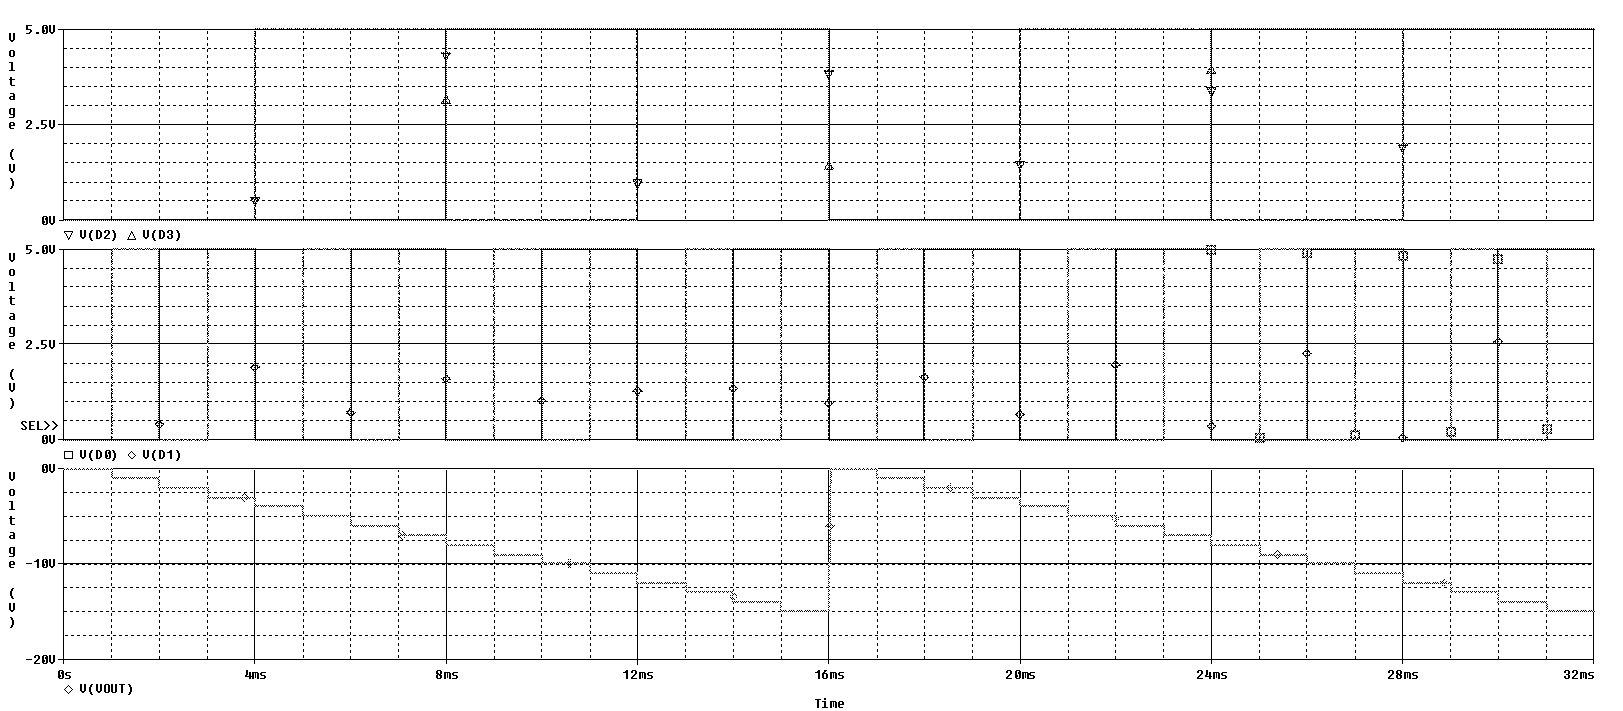
\includegraphics[width=.8\textwidth]{img/plot/part1_plot2b.PNG}
	\parbox{.8\textwidth}{
	\caption[Discrete DAC --- Tuned Results]{Final simulation results with an
	adjusted feedback resistor.}
	\label{f:dac_plot2}}
\end{figure}

\subsection{Discrete DAC Results}
As is shown in the above included PSpice plot, the digital to analog converter
produces an accurate representation of the input bits.  By adjusting the value
of the feedback resistor, students were able to ensure that the full-scale
input produced an output voltage within the range of values that could be
accurately represented.  The supply voltages for the operational amplifier
determined the maximum and minimum possible outputs, thus requiring students to
force a full-scale input of~$0000_2$ to~\SI{-15}{\volt} or more.  The output
waveform shows that for each increase in input value there is a corresponding
decrease in output voltage, a voltage difference that remains constant through
the entire range of inputs at roughly~\SI{-1}{\volt\per\bit}.

\section{Analog to Digital Converter}
\subsection{Discrete ADC Simulation}
The initial stage of the voice recording circuit is an analog to digital
converter allowing the digital storage system to process the analog input from
an eletret microphone.  A simplified ADC schematic was provided in the lab
instructions, and was simulated with Cadence PSpice as shown in
Figure~\ref{f:adc_schem}.
%
\begin{figure}[H]
\centering
	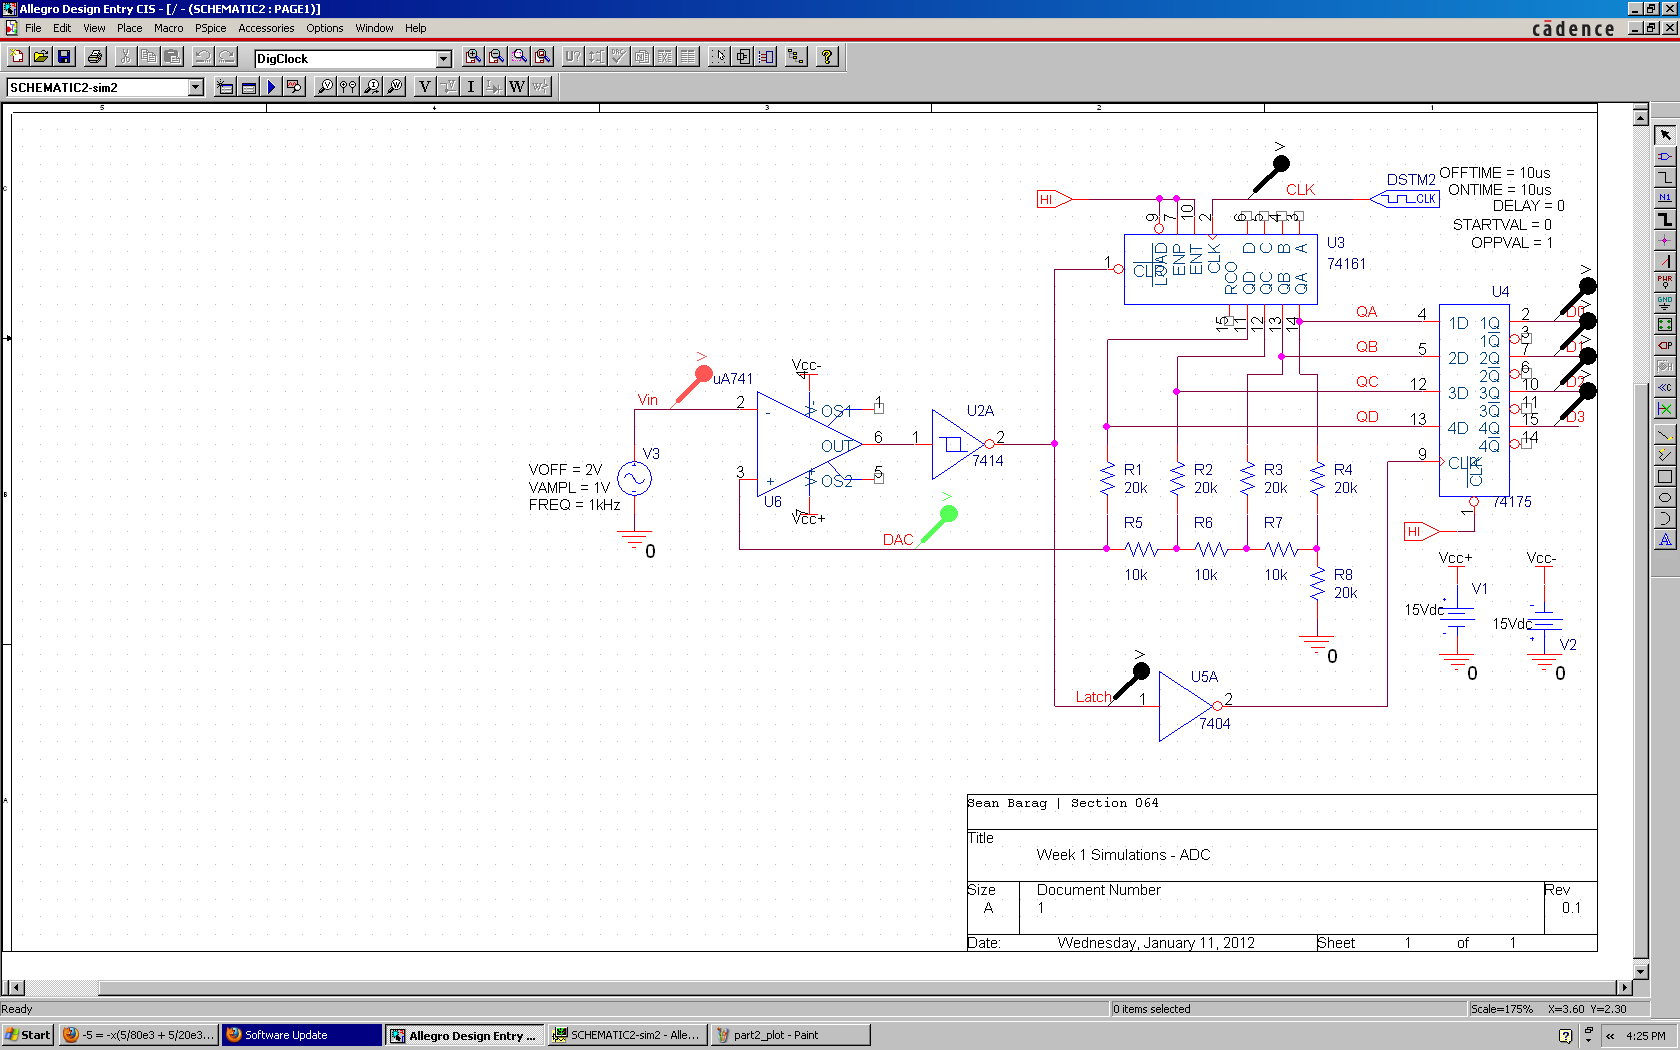
\includegraphics[width=.8\textwidth]{img/shot/part2_schem.PNG}
	\parbox{.8\textwidth}{
	\caption[Discrete ADC --- Schematic]{Schematic for the simplified ADC
	provided by the lab instructions.}
	\label{f:adc_schem}}
\end{figure}
%
This circuit was simulated using transient analysis lasting for
just~\SI{2}{\milli\second}.  Because of the~\SI{1}{\kilo\hertz} frequency of
the sinusoidal input signal, the system will be observed for two full input
periods, as shown in Figure~\ref{f:adc_plot}.

\subsection{Discrete ADC Results}
Upon the completion of the transient simulation, PSpice produced the plot
included in Figure~\ref{f:adc_plot}.
%
\begin{figure}[H]
\centering
	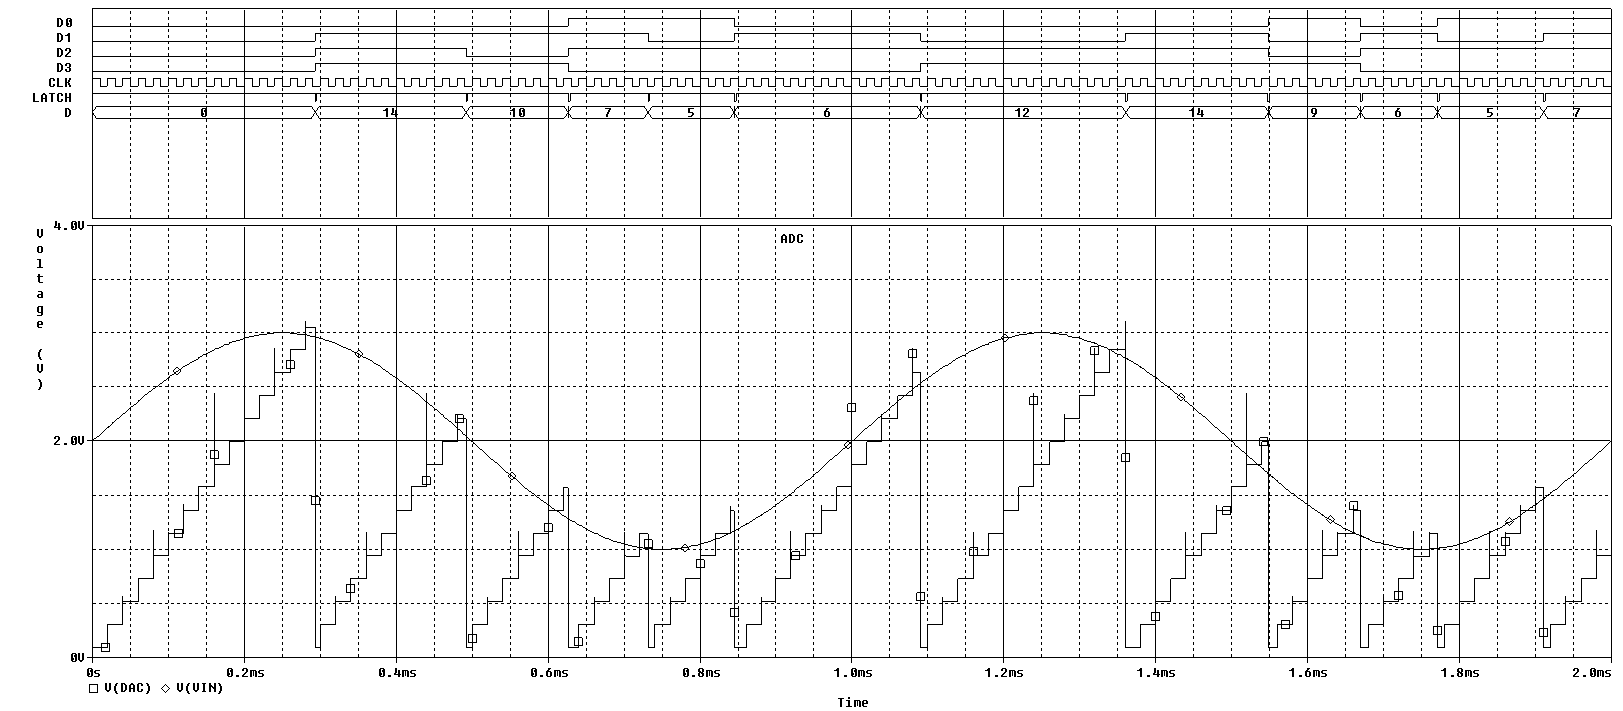
\includegraphics[width=.8\textwidth]{img/plot/part2_plot.PNG}
	\parbox{.8\textwidth}{
	\caption[Discrete ADC --- Results]{PSpice-produced plot of the input
	voltage and output voltages, as well as the voltages at the ``Latch'' and
	``Clk'' nodes as indicated above.}
	\label{f:adc_plot}}
\end{figure}
%
The plot reveals a lot of information about the function of this particular
ADC.  The value of the DAC line increases in discrete steps due to the binary
counter U3.  When the voltage on this line exceeds the input voltage, the latch
line goes low and triggers the D flip-flop U4 to produce the corresponding
digital bits D0 through D3.  At this point, the counter resets, latch goes
high, and the counting process repeats.  While this does provide accurate
digital representations of individual signals, it causes the rate of
measurement to increase for inputs with larger voltages as each value in the
count up process is analyzed for one clock period (in this
case~\SI{20}{\micro\second}).

\section{Integrated Circuit ADC/DAC}
\subsection{High Voltage, Low Frequency}
Also included in the lab instructions was a schematic for a combined ADC/DAC
circuit in which the outputs of an analog to digital converter is fed
immediately into the inputs of a digital to analog converter.  This allows
students to observe the overall accuracy of the ADC and DAC when pipelined, as
well as observing how well the system reproduces an arbitrary input.  A PSpice
capture of this schematic is shown in Figure~\ref{f:combined_schem}.
%
\begin{figure}[H]
\centering
	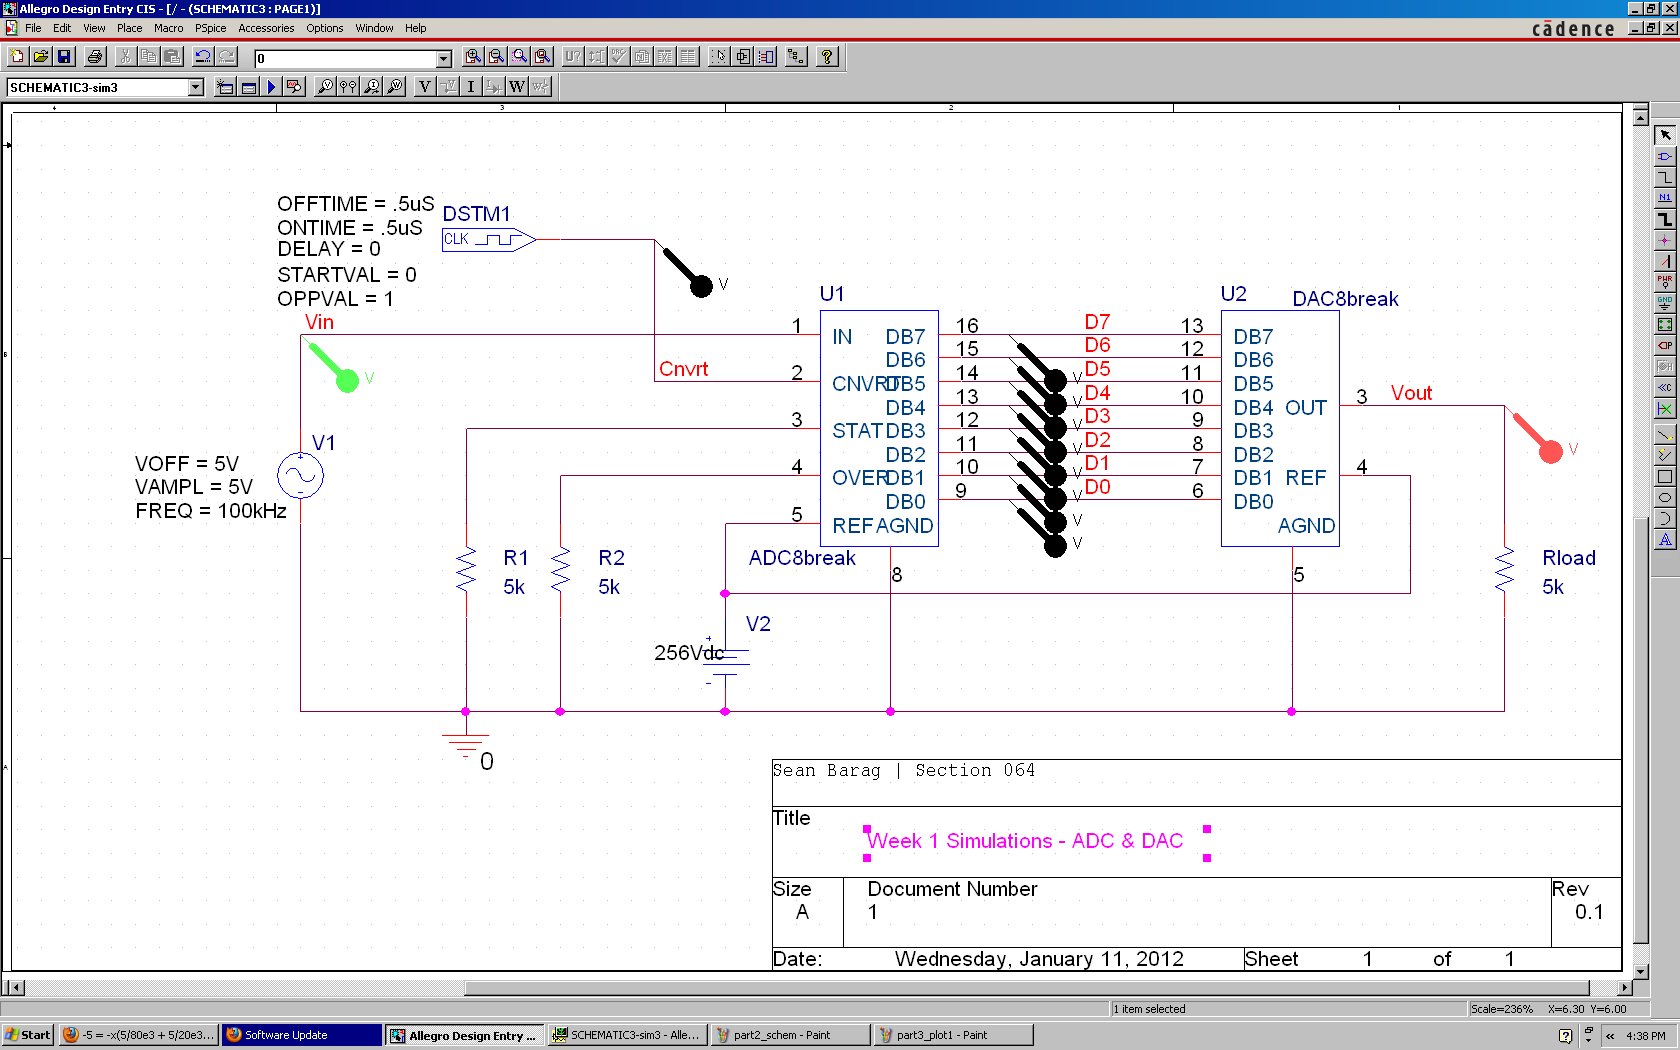
\includegraphics[width=.8\textwidth]{img/shot/part3_schem.PNG}
	\parbox{.8\textwidth}{
	\caption[Integrated Circuit --- Schematic]{Instructor provided schematic
	for the integrated circuit ADC/DAC.  Note that there are absolutely no
	elements between the outputs of the ADC and the inputs of the DAC.  This
	represents an idealized case that is not relevant in the final voice
	recorder design.}
	\label{f:combined_schem}}
\end{figure}
%
The circuit was simulated using a transient analysis
over~\SI{20}{\micro\second}, allowing the sinusoidal input to complete two full
periods.  After the simulation completed, PSpice produced the plot in
Figure~\ref{f:combined_plot1}.
%
\begin{figure}[H]
\centering
	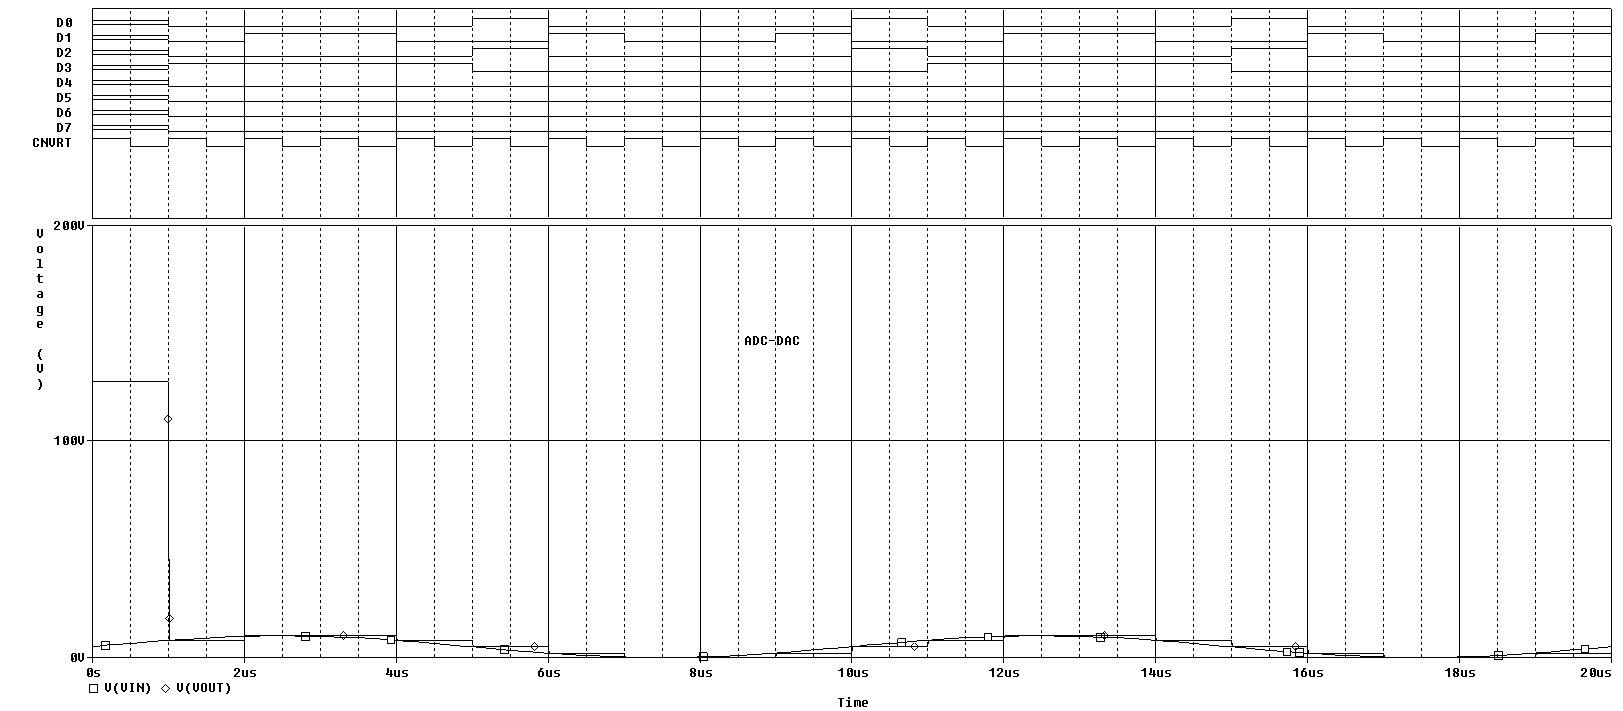
\includegraphics[width=.8\textwidth]{img/plot/part3_plot1.PNG}
	\parbox{.8\textwidth}{
	\caption[Integrated Circuit --- Initial Results]{PSpice-generated plot of
	the initially simulated integrated circuit (IC) ADC/DAC.}
	\label{f:combined_plot1}}
\end{figure}
%
Note that the time resolution of the system's output is dependant on the clock
frequency provided to the ADC.  In this configuration, the output can only
change once every microsecond.

\subsection{Low Voltage, High Frequency}
The output voltage of the DAC is determined by an equation very similar
to~\eqref{eq:dac}, as shown in~\eqref{eq:dac_ic}.
%
\begin{equation}
	V_\text{out} = V_\text{ref} \left[
		\frac{D_0}{256} +
		\frac{D_1}{128} +
		\frac{D_2}{64}  +
		\frac{D_3}{32}  +
		\frac{D_4}{16}  +
		\frac{D_5}{8}   +
		\frac{D_6}{4}   +
		\frac{D_7}{2} \right]
	\label{eq:dac_ic}
\end{equation}
%
In the case of a full-scale input to the DAC of~$11111111_2$, the output in
this configuration would be~$\SI{256}{\volt} \cdot \frac{255}{256} =
\SI{255}{\volt}$ --- a value that is far too large to be safely used for small
scale audio applications.  The reference voltage for the system was tuned
using~\eqref{eq:dac_ic} so that the full scale output of the DAC would be
roughly~\SI{10}{\volt}.  This resulted in a calculated reference voltage
of~\SI{10.0392157}{\volt}.  The clock frequency was also increased
from~\SI{1}{\mega\hertz} to~\SI{10}{\mega\hertz} as per the lab instructions.

Once the system was reconfigured, the~\SI{20}{\micro\second} transient analysis
was repeated, producing the plot in Figure~\ref{f:combined_plot2}.
%
\begin{figure}[H]
\centering
	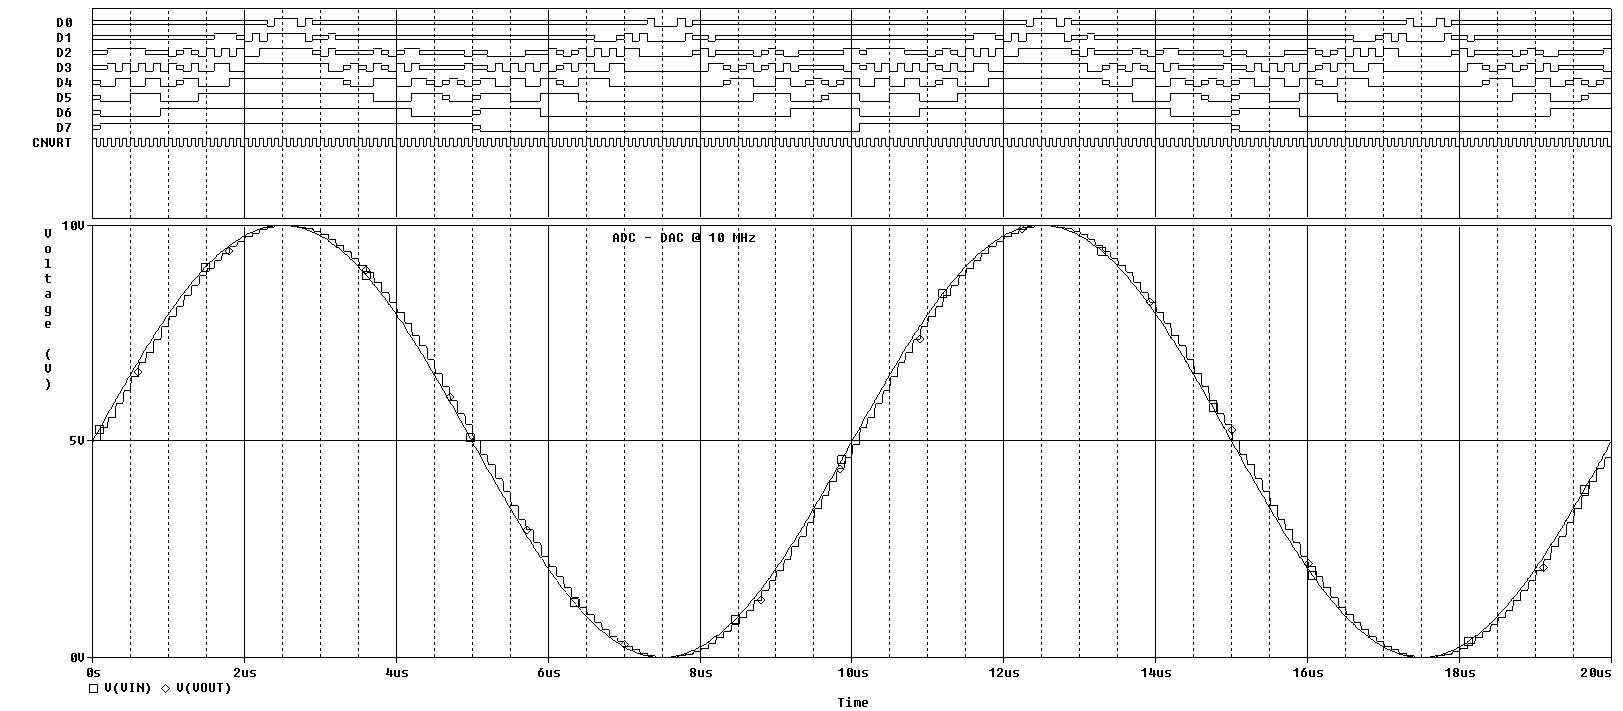
\includegraphics[width=.8\textwidth]{img/plot/part3_plot2.PNG}
	\parbox{.8\textwidth}{
	\caption[Integrated Circuit --- Tuned Results]{Plot of the tuned IC ADC/DAC
	as simulated by Cadence PSpice.  Note that the output is now limited
	to~\SI{10}{\volt} maximum, as compared to the high-voltage system shown in
	Figure~\ref{f:combined_plot1}.}
	\label{f:combined_plot2}}
\end{figure}
%
As with the high-voltage configuration, the system's time resolution is
dependant on the clock frequency feeding the ADC.  For the reconfigured system,
the time resolution is just~\SI{100}{\nano\second}.  This is evident in
Figure~\ref{f:combined_plot2}, as the output waveform more closely matches the
input than in the high-voltage case.


\newpage
\appendix
\section{License}
\section{License}

Copyright \copyright\ 2011, Sean Barag.  All rights reserved.

Redistribution and use in source and binary forms, with or without
modification, are permitted provided that the following conditions are met:
\begin{itemize}
\item Redistributions of source code must retain the above copyright notice, this
  list of conditions and the following disclaimer.
\item Redistributions in binary form must reproduce the above copyright notice, this
  list of conditions and the following disclaimer in the documentation and/or
  other materials provided with the distribution.
\item Neither the name of the owner nor the names of its contributors may be
  used to endorse or promote products derived from this software without specific
  prior written permission.
\end{itemize}

THIS SOFTWARE IS PROVIDED BY THE COPYRIGHT HOLDERS AND CONTRIBUTORS ``AS IS'' AND
ANY EXPRESS OR IMPLIED WARRANTIES, INCLUDING, BUT NOT LIMITED TO, THE IMPLIED
WARRANTIES OF MERCHANTABILITY AND FITNESS FOR A PARTICULAR PURPOSE ARE
DISCLAIMED. IN NO EVENT SHALL THE COPYRIGHT HOLDER OR CONTRIBUTORS BE LIABLE
FOR ANY DIRECT, INDIRECT, INCIDENTAL, SPECIAL, EXEMPLARY, OR CONSEQUENTIAL
DAMAGES (INCLUDING, BUT NOT LIMITED TO, PROCUREMENT OF SUBSTITUTE GOODS OR
SERVICES; LOSS OF USE, DATA, OR PROFITS; OR BUSINESS INTERRUPTION) HOWEVER
CAUSED AND ON ANY THEORY OF LIABILITY, WHETHER IN CONTRACT, STRICT LIABILITY,
OR TORT (INCLUDING NEGLIGENCE OR OTHERWISE) ARISING IN ANY WAY OUT OF THE USE
OF THIS SOFTWARE, EVEN IF ADVISED OF THE POSSIBILITY OF SUCH DAMAGE.\\

Source code for this document is available at \texttt{http://github.com/sjbarag/}.


\end{document}
